\documentclass{article}
\usepackage[margin=0.65in]{geometry}
\usepackage{enumitem}
\usepackage{graphicx}
\usepackage{hyperref}
\usepackage{titlesec}
\usepackage{xcolor}
\hypersetup{hidelinks}
\setlist[itemize]{leftmargin=1.5em,topsep=2pt,itemsep=1pt,parsep=0pt,partopsep=0pt}
\titlespacing*{\section}{0pt}{1.2ex}{0.6ex}
\setlength{\parindent}{0pt}
\setlength{\parskip}{0.5em}
\setlength{\textfloatsep}{8pt}
\setlength{\intextsep}{6pt}
\setlength{\abovecaptionskip}{4pt}
\setlength{\belowcaptionskip}{0pt}
\makeatletter
\renewcommand{\maketitle}{%
    \begin{center}
        {\Large\bfseries \@title\par}\vspace{0.1em}
        {\normalsize \@author\par}\vspace{0.1em}
        {\small \@date\par}
    \end{center}\vspace{0.4em}
}
\makeatother
% HJNotes-Tags: AI Infra, Speculative Decoding, KL Divergence, Cross Entropy
% HJNotes-Summary: KL divergence vs cross entropy (and their one-hot simplification), plus the shift-by-1 used when the target model verifies draft tokens in speculative decoding.
% AGENT WARNING: Polish task shouldn't delete or add new stuff unless there are serious mistake. typo should be fixed at once, permission is not needed.
\title{Speculative Decoding}
\author{HJ}
\begin{document}
\maketitle
\section{Foundamental Math}
\subsection{KL divergence}
$D_{\mathrm{KL}}(P\,\|\,Q)$ measures how much a distribution $Q$ diverges from a reference distribution $P$: the expectation, under $P$, of the log-ratio $\log\frac{P(x)}{Q(x)}$.
\[
D_{\mathrm{KL}}(P\,\|\,Q) \;=\; \sum_x P(x)\log\frac{P(x)}{Q(x)}.
\]
It is non-negative, equals $0$ iff $P=Q$, and is asymmetric, so it is a divergence rather than a true distance. In ML it is used to quantify how far a model's predicted distribution $Q$ is from the true distribution $P$.

\subsection{Cross entropy}
$H(P,Q)$ is the expected $-\log Q(x)$ under the true distribution $P$---intuitively, how ``surprised'' samples drawn from $P$ are under the model's distribution $Q$:
\[
H(P,Q) \;=\; -\sum_x P(x)\log Q(x).
\]
Writing the entropy of $P$ as $H(P)=-\sum_x P(x)\log P(x)$, the three quantities satisfy
\[
H(P,Q) \;=\; H(P) + D_{\mathrm{KL}}(P\,\|\,Q),
\]
i.e.\ cross entropy is the true entropy plus the extra cost of using $Q$ instead of $P$. Since $H(P)$ does not depend on $Q$, minimizing cross entropy is equivalent to minimizing KL divergence, which is why cross entropy is the standard classification loss.

\textbf{The one-hot case.} In classification and next-token prediction the label is a single class/token, so the true distribution $P$ is a one-hot vector: $P(c)=1$ for the correct class $c$, $0$ elsewhere. Then $H(P)=0$, and:
\[
H(P,Q) \;=\; D_{\mathrm{KL}}(P\,\|\,Q) \;=\; -\log Q(c) \;=\; \log\sum_j e^{z_j} - z_c,
\]
where $Q=\mathrm{softmax}(z)$, z is logits.

\section{Fast Speculative Decoding}
\begin{figure}[!ht]
    \centering
    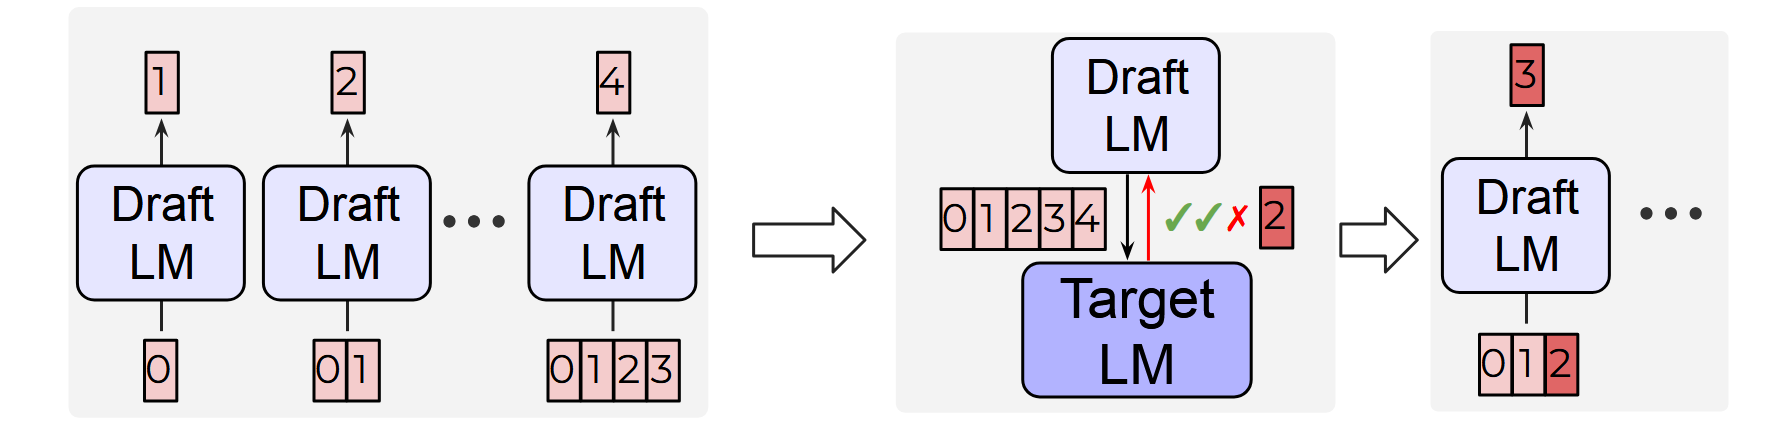
\includegraphics[width=\linewidth,height=0.52\textheight,keepaspectratio]{speculative-decoding.png}
    \caption{Speculative Deocoding Procedure.}
\end{figure}

\subsection{Shift by 1 when verifying}
When the target model verifies, input token ids \texttt{iL} are $[B,L]$ and output logits \texttt{oL} are $[B,L,V]$; \texttt{oL[i]} predicts the next token after \texttt{iL[i]}, so the label to verify is \texttt{iL[i+1]}. Hence the shift-by-1 pairs \texttt{oL[:-1]} with \texttt{iL[1:]}.

\subsection{TODO}
\textcolor{red}{Might add after I fully grasp the math of paper}

\end{document}

